% Below is your UAH LaTeX template. This is the main file that compiles your document. You will need to fill out the appropriate sections below.
\documentclass[oneside, 12pt]{book} % Document class


\usepackage[utf8]{inputenc} % Basic package for Latex
%\usepackage[draft]{graphicx} % To help include figures
\usepackage{listings}
\lstset{basicstyle=\ttfamily}
\usepackage{graphicx} % To help include figures
\usepackage{geometry} % To allow document margin changes
\usepackage{setspace} % To allow custom spacing
\usepackage{indentfirst} % To allow indentations in the first paragraph.
\usepackage{amsmath} % For formatting equations properly
\usepackage{natbib} % For formatting the bibliography
\usepackage{chngcntr} % To allow changing how figures, tables, and pages are counted.
\usepackage{appendix} % To help format the appendix
\usepackage[font=small,labelfont=bf]{caption} %This makes caption font small and makes the caption heading bold.
\usepackage{tabularx} %To allow formatting Tables.
\usepackage{array} %To allow creating arrays.
\usepackage{multirow, tabularx}
\usepackage{multicol}
\usepackage{physics}
\providecommand\phantomsection{} %This command allows you to make phantom sections that have no title but are still included in the Table of Contents such as the epigraph.
\usepackage[all]{nowidow} %This prevents widow/orphan lines
\usepackage{tikz}%This package helps to anchor the seal on the title page to the student name
\usetikzlibrary{tikzmark}%This is part of the tikz package


%Creating an Interlude Environment in order to NOT count or number a certain page such as the copyright page.
\newenvironment{interlude}{
  \clearpage
  \thispagestyle{empty}% we want this page to be empty (adjust to use a modified page style)
  \pagestyle{empty}% use the same style for subsequent pages in the unnumbered section
  }
  {\clearpage}

%The following package and lines can be used to format and create a list of symbols, equations, abbreviations, etc. The example actually used in this template is the \glossaries package, but you may also use this \nomencl package if desired.
\usepackage[intoc]{nomencl}
\makenomenclature
\renewcommand{\nomname}{List of Symbols}

% This is to ensure the page numbers are centered and at the bottom.
\usepackage{fancyhdr}
\pagestyle{fancy}
\fancyhf{}
\renewcommand{\headrulewidth}{0pt}
\cfoot{\thepage}

%This defines a new page style for just the title page.
\fancypagestyle{logopage}{\fancyhf{}\renewcommand{\headrulewidth}{0pt}\fancyfoot[C]{\includegraphics[scale=0.3]{Figures/Color Grad Banner.png}}}

%this causes equations to be counted according to their chapter location
\counterwithin{equation}{chapter} %this causes equations to be counted according to their chapter location
\counterwithin{figure}{chapter}




%This formats the table of contents the way Dr. Hakkila wants it
\usepackage[titles]{tocloft}


%Removes the Duplicate Chapter
\setcounter{secnumdepth}{4}% Show down to subsubsection

\setlength{\cftchapindent}{-20pt}% Just some value...

\usepackage{xpatch}

\makeatletter
\xpatchcmd{\@chapter}{\addcontentsline{toc}{chapter}{\protect\numberline{\thechapter}#1}}{%
                      \addcontentsline{toc}{chapter}{\protect\numberline{}#1}}{\typeout{Success}}{\typeout{Failed!}}
\makeatother



%This formats the Table of contents title
\renewcommand{\contentsname}{\hspace*{\fill}\bfseries\large Table of Contents\hspace*{\fill}}


\renewcommand{\cftbeforetoctitleskip}{-0.25in}

\renewcommand\cftchapdotsep{\cftdotsep}
\renewcommand\cftchapleader{\cftdotfill{\cftchapdotsep}}
%\renewcommand{\cftchappresnum}{CHAPTER } % put this before the number
%\addtolength{\cftchapnumwidth}{6em} % extra space for number and pre-name
%\renewcommand{\cftchapaftersnum}{. } % put period after chapter number and space


%This puts all the chapter headings into all-caps
%\renewcommand{\chaptername}{CHAPTER}

%Hopefully this reformats the List of Figures Title
\renewcommand{\listfigurename}{\hspace*{\fill}\bfseries\large List of Figures\hspace*{\fill}}

%Reformat List of Tables, etc.
\renewcommand{\listtablename}{\hspace*{\fill}\bfseries\large List of Tables\hspace*{\fill}}


%This creates a List of Equations.
\newcommand{\listequationsname}{List of Equations}
\newlistof{equations}{equ}{\listequationsname}

\newcommand{\eqdesc}[1]{%
  \csname phantomsection\endcsname % if hyperref is loaded
  \addcontentsline{equ}{equations}{\protect\numberline{\theequation}#1}%
}

\setlength{\parindent}{36pt}


%The following formats the chapter titles and sections appropriately
\usepackage{titlesec}



\titleformat
{\chapter}
[hang]
{\normalfont\large\bfseries\filcenter}
{} %Label. This is blank so that the entire chapter heading and title are properly centered.
{0pt} %  Horizontal Space between label and title body.
{} %Before-Code
{}

\titleformat
{\section}
[hang]
{\normalfont\normalsize\bfseries}
{\thetitle} %Label.
{.5em} %  Horizontal Space between label and title body.
{} %Before-Code
{}

\titleformat
{\subsection}
[hang]
{\normalfont\normalsize\bfseries}
{\thetitle} %Label.
{.5em} %  Horizontal Space between label and title body.
{} %Before-Code
{}

\titlespacing{\subsection}{2em}{12pt}{12pt}

\titlespacing{\chapter}{0pt}{50pt}{12pt}

\titlespacing{\part}{0pt}{12pt}{12pt}


\titlespacing{name=\chapter, numberless}{0pt}{0pt}{12pt}


% I had used this code to combine the chapter heading and
%\titleformat{\chapter}[hang]
 % {\normalfont\large\bfseries\filcenter}{\chaptertitlename\ \thechapter:}{.3em}{}


%This names the Bibliography/References whatever you want it to be.
\renewcommand{\bibname}{References}

%The below package creates the optional List of Symbols and formats it correction..
\usepackage[acronyms, automake, toc, nopostdot]{glossaries}
\usepackage{glossary-longbooktabs}
\newcolumntype{P}[1]{>{\centering\arraybackslash}p{#1}}
\renewcommand*{\entryname}{Symbol}
\newglossarystyle{mystyle}{% define custom glossaries style for Abbreviation page, read relative manual before change
\setglossarystyle{long-booktabs}%
\renewenvironment{theglossary}%
{\begin{longtable}{@{}P{3cm}@{}p{\dimexpr\linewidth-3cm}@{}}}%
{\end{longtable}}%

\renewcommand*{\glossaryheader}{%
 \bfseries\large Symbol & \centering\bfseries\large Description \tabularnewline\endhead \endfoot}%
}

\renewcommand{\glossarypreamble}{\normalsize}
\makeglossaries
 %To clean up this document, the preamble that includes the packages is located in the preamble.tex file found in the FrontMatter folder.

%********************************************
%********************************************
% THE SECTION BELOW MUST BE FILLED OUT
%********************************************
%********************************************

%BASIC INFORMATION
\newcommand{\thesistitle}{Deep Learning Time Series Prediction Strategies for Efficiently Emulating Noah Land Surface Model Soil Moisture Dynamics}
\newcommand{\studentname}{Mitchell T. Dodson}
\newcommand{\degree}{Master of Science in Atmospheric Science}
\newcommand{\department}{Atmospheric and Earth Science}
\newcommand{\gradyear}{2025}% complete 4 digit year, e.g., 2022
\newcommand{\gradmonth}{May}% Spell out the month completely, e.g., December
%\newcommand{\jointuni}{Auburn University} %If this is a joint degree, remove the % sign at the beginning of this line and enter the entire name of the additional universities.

%***********************
%SPECIFY THESIS OR DISSERTATION
% Below, if you are earning a master's degree, remove the "%" on the line below that says \newcommand{thesis}. If you are earning a PhD or other doctorate degree, remove the "%" on the line below that says \newcommand{dissertation}.

\newcommand{\thesis}{FOR MASTER'S STUDENTS ONLY}
%\newcommand{\dissertation}{FOR DOCTORATE DEGREE STUDENTS ONLY}

%*******************************
%SPECIFY THE PROFESSORS WHO WILL APPROVE YOUR THESIS/DISSERTATION
%Professor information: Fill out only their first and last name WITH NO PREFIXES OR SUFFIXES. If a line is not applicable, simply add a % sign at the beginning of that line. If there is an applicable line that has a % sign at the beginning, remove this sign and fill in as needed.
\newcommand{\resadv}{Christopher Hain}
\newcommand{\comchair}{Sundar Christopher}
%\newcommand{\reschair}{Research Advisor/Committee Chair Name} %If your research advisor and committee chair are the same person, enter his/her name on this line.
\newcommand{\commema}{Sean Freeman}
%\newcommand{\commemb}{[2nd Committee Member Name]}
%\newcommand{\commemc}{[3rd Committee Member Name]}
%\newcommand{\commemd}{[4th Committee Member Name]}
%\newcommand{\commeme}{[5th Committee Member Name]}
%\newcommand{\commemf}{[6th Committee Member Name]}
%\newcommand{\commemg}{[7th Committee Member Name]}
%\newcommand{\commemh}{[8th Committee Member Name]}
%\newcommand{\commemi}{[9th Committee Member Name]}
\newcommand{\depchair}{Lawrence Carey}
\newcommand{\colldean}{[College Dean Name]}
\newcommand{\graddean}{Jon Hakkila}

%**************
%INDICATE IF YOU HAVE REGISTERED FOR A COPYRIGHT.
%**************
%\newcommand{\copyrightreg}{Yes} %If you registered for a copyright through Proquest, please remove the % sign from the beginning of this line starting with \newcommand{\copyrightreg}{Yes}. If you did not register for a copyright, no action is needed.

%********************************************
%********************************************
% End of Section to Fill Out.
%********************************************
%********************************************

%This creates hyperlinks for chapter, figure, and table titles in your pdf. It should be the last package before the document begins.
\usepackage[colorlinks=true,linkcolor=black,anchorcolor=black,citecolor=black,filecolor=black,menucolor=black,runcolor=black,urlcolor=black]{hyperref}

%*********************************************
%*********************************************
%Optional List of Symbols/Abbreviations
%*********************************************
%*********************************************

%A list of symbols/abbreviations is optional. If you do not want to include one, simply delete this section from your document. You may also delete this section and use a different package as there are multiple packages that can be used to make a List of Symbols, Abbreviations, Nomenclature, Etc. Below uses the \glossaries-extra package. This package is nice if you want to include multiple lists or sections. The following links provide useful information on how to use this package.
% https://mirrors.mit.edu/CTAN/macros/latex/contrib/glossaries/glossariesbegin.pdf
% https://mirrors.rit.edu/CTAN/macros/latex/contrib/glossaries/glossaries-user.pdf
% https://www.overleaf.com/learn/latex/Glossaries


% This uses the glossaries package. With this package, you can include multiple types of lists, track page numbers if desired, and define new lists. More information can be found at the following sites: https://mirrors.mit.edu/CTAN/macros/latex/contrib/glossaries/glossariesbegin.pdf and https://mirrors.rit.edu/CTAN/macros/latex/contrib/glossaries/glossaries-user.pdf https://www.overleaf.com/learn/latex/Glossaries


%*****************************************
%Define your list of glossary items below. Remember that the entries that you enter in this file will not automatically appear in the List of Symbols. You also have to reference the symbol in the body of your thesis by using the \gls command. 

%symbols
\newglossaryentry{deg}{name=$^\circ$, description={Degree}}
\newglossaryentry{grav}{name={1D}, description={Normal gravity environment}}
\newglossaryentry{wf}{name={\textit{f}}, description={Wear factor}}
\newglossaryentry{alp}{name={$\alpha$},description={Alpha}}
\newglossaryentry{theta}{name={$r_O$}, description={ecosystem respiration at reference temperature $T_a=0{^\circ}$C}}
\newglossaryentry{te}{name={$\tau_e$}, description={precision of the normal distribution of the likelihood}}
\newglossaryentry{q10}{name={$Q_{10}$}, description={multiplication factor to respiration with 10$^\circ$C increases in $T_a$}}
\newglossaryentry{phi}{name={$\phi$}, description={vapour pressure deficit response function}}
\newglossaryentry{del}{name=$\delta$, description={Transition coefficient constant for the design of linear-phase FIR filters which are used to take up space when testing the list of symbols}}

 %Go to this page to enter all the symbols you plan to use in the document.

% Scroll down in this file to after the List of Tables section in order to actually add your Lists to your document,.

%**********************************************
%**********************************************
% End of Optional List of Symbols/Abbreviations
%**********************************************
%**********************************************



%******************************************
%******************************************
% Document Begins Here
%******************************************
%******************************************

\begin{document}

\frontmatter % This command creates the front matter environment.

%**********************************
%**********************************
%Title Page
%**********************************
%**********************************
% Do not directly edit this page. Everything on the Title Page should auto-fill if you correctly filled out the information on the main.tex file.

\begin{titlepage}
\newgeometry{left=1.5in,bottom=.5in}
    \begin{center}
        \Large
        \singlespacing
        \textbf{\thesistitle}
        

\vspace{2cm}

        \large
        \textbf{\studentname}\\
        \vspace{1.5cm}
        \normalsize
        \ifdefined\thesis
        \textbf{A THESIS}
        \vspace{1.5cm}
        \else
        \ifdefined\dissertation
        \textbf{A DISSERTATION}
        \vspace{1.5cm}
        \else
        Please identify this document as either a thesis or dissertation on the main.tex file in the section at the top that must be filled out.
        \vspace{1.5cm}
        \fi
        \fi

        \textbf{Submitted in partial fulfillment of the requirements \\for the degree of \degree}\\  
        
\vspace{0.1cm}
  \textbf{in}\\
      \vspace{0.1cm}
        \textbf{The Department of \department}\\
        \vspace{0.1cm}
  \textbf{to}\\
\vspace{0.1cm}
\textbf{The Graduate School}\\
\vspace{0.1cm}
\textbf{of}\\
\vspace{0.1cm}
        \ifdefined\jointuni
        \textbf{The University of Alabama in Huntsville\\ and\\  \jointuni}
        \else
        \textbf{The University of Alabama in Huntsville}
    \fi

        
        \vspace{0.4cm}
        \textbf{\gradmonth\ \gradyear}
        


    \end{center}
    

\vfill

\textbf{Approved by:}


\vspace{.1cm}
\setstretch{1.25}

\ifdefined\reschair
\noindent
Dr. \reschair, Research Advisor/Committee Chair\\
\else
\noindent
Dr. \resadv, Research Advisor \\
Dr. \comchair, Committee Chair\\
\fi
\ifdefined\commemi
\noindent
Dr. \commema, Committee Member\\
Dr. \commemb, Committee Member\\
Dr. \commemc, Committee Member\\
Dr. \commemd, Committee Member\\
Dr. \commeme, Committee Member\\
Dr. \commemf, Committee Member\\
Dr. \commemg, Committee Member\\
Dr. \commemh, Committee Member\\
Dr. \commemi, Committee Member\\
Dr. \depchair, Department Chair\\
Dr. \colldean, College Dean\\
Dr. \graddean, Graduate Dean\\
\else
\ifdefined\commemh
\noindent
Dr. \commema, Committee Member\\
Dr. \commemb, Committee Member\\
Dr. \commemc, Committee Member\\
Dr. \commemd, Committee Member\\
Dr. \commeme, Committee Member\\
Dr. \commemf, Committee Member\\
Dr. \commemg, Committee Member\\
Dr. \commemh, Committee Member\\
Dr. \depchair, Department Chair\\
Dr. \colldean, College Dean\\
Dr. \graddean, Graduate Dean\\
\else
\ifdefined\commemg
\noindent
Dr. \commema, Committee Member\\
Dr. \commemb, Committee Member\\
Dr. \commemc, Committee Member\\
Dr. \commemd, Committee Member\\
Dr. \commeme, Committee Member\\
Dr. \commemf, Committee Member\\
Dr. \commemg, Committee Member\\
Dr. \depchair, Department Chair\\
Dr. \colldean, College Dean\\
Dr. \graddean, Graduate Dean\\
\else
\ifdefined\commemf
\noindent
Dr. \commema, Committee Member\\
Dr. \commemb, Committee Member\\
Dr. \commemc, Committee Member\\
Dr. \commemd, Committee Member\\
Dr. \commeme, Committee Member\\
Dr. \commemf, Committee Member\\
Dr. \depchair, Department Chair\\
Dr. \colldean, College Dean\\
Dr. \graddean, Graduate Dean\\
\else
\ifdefined\commeme
Dr. \commema, Committee Member\\
Dr. \commemb, Committee Member\\
Dr. \commemc, Committee Member\\
Dr. \commemd, Committee Member\\
Dr. \commeme, Committee Member\\
Dr. \depchair, Department Chair\\
Dr. \colldean, College Dean\\
Dr. \graddean, Graduate Dean\\
\else
\ifdefined\commemd
Dr. \commema, Committee Member\\
Dr. \commemb, Committee Member\\
Dr. \commemc, Committee Member\\
Dr. \commemd, Committee Member\\
Dr. \depchair, Department Chair\\
Dr. \colldean, College Dean\\
Dr. \graddean, Graduate Dean\\
\else
\ifdefined\commemc
Dr. \commema, Committee Member\\
Dr. \commemb, Committee Member\\
Dr. \commemc, Committee Member\\
Dr. \depchair, Department Chair\\
Dr. \colldean, College Dean\\
Dr. \graddean, Graduate Dean\\
\else
\ifdefined\commemb
Dr. \commema, Committee Member\\
Dr. \commemb, Committee Member\\
Dr. \depchair, Department Chair\\
Dr. \colldean, College Dean\\
Dr. \graddean, Graduate Dean\\
\else
\ifdefined\commema
Dr. \commema, Committee Member\\
Dr. \depchair, Department Chair\\
Dr. \colldean, College Dean\\
Dr. \graddean, Graduate Dean\\
\else
Dr. \depchair, Department Chair\\
Dr. \colldean, College Dean\\
Dr. \graddean, Graduate Dean\\
\fi
\fi
\fi
\fi
\fi
\fi
\fi
\fi
\fi
\end{titlepage}


\restoregeometry%Your title page should self-generate after filling in the required information above.
\newpage

%This sets the page margins. If you plan to bind and print your thesis, change the left boarder to 1.5 in.
\newgeometry{left=1.5in, right=1in, bottom=1in, top=1in}
\setcounter{page}{2}
%**********************************
%**********************************
%Abstract Page
%**********************************
%**********************************

%The below code inserts your Abstract Page. While much of this page fills in automatically, you must go to the AbstractPage.tex file located in the FrontMatter folder and insert the actual text of your abstract.

% The top of your abstract will fill out automatically once you fill in the required fields on the main.tex file. In this file, you will provide your abstract body. Type your abstract body at the bottom of this page directly below the \doublespacing command.

\chapter{Abstract}
     \begin{center}
        \large
        \singlespacing
        \textbf{\thesistitle}\\
        \vspace{0.5cm}
        \large
        \textbf{\studentname}\\
        \vspace{0.5cm}
        \normalsize
        \ifdefined\thesis
        \textbf{A thesis submitted in partial fulfillment of the requirements \\for the degree of \degree}\\
        \else
        \ifdefined\dissertation
        \textbf{A dissertation submitted in partial fulfillment of the requirements \\for the degree of \degree}\\
        \else
        \textbf{Please identify this document as either a thesis or dissertation on the main.tex in the section at the top that must be filled out.}\\
    \fi
    \fi
        \vspace{1cm}
        \textbf{\department}

        \vspace{0.25cm}

        \ifdefined\jointuni
        \textbf{The University of Alabama in Huntsville and  \jointuni}
        \else
        \textbf{The University of Alabama in Huntsville}
    \fi


        \vspace{0.1cm}
        \textbf{\gradmonth\ \gradyear}



    \end{center}
\vspace{0.1cm}

%****************************************************
%Enter the body of your abstract below. Remember there is a 150 word limit!
%****************************************************
\doublespacing

This work examines the ability of deep learning time series generative models to accurately and efficiently emulate the hourly temporal dynamics of the Noah Land Surface Model (Noah-LSM) out to a 2 week forecast horizon, given atmospheric forcings and static parameterization provided by the second phase North American Land Data Assimilation System (NLDAS-2) framework. Results from multiple neural network architectures are compared alongside variations in prediction target, loss function characteristics, and model properties. The most performant model types are subsequently evaluated with respect to forecast distance, daily and annual seasonality, and against a variety of regional scenarios, including several extreme event case studies. Ultimately, we present a software system for developing and testing neural networks that use time-varying and static data to estimate temporal dynamics, with the goal of providing a foundation for similar data-driven modeling techniques to be implemented within the upcoming third phase of the NLDAS data record.

\clearpage



%**********************************
%**********************************
%Copyright Page
%**********************************
%**********************************

% The following code inserts your COPYRIGHT page. If you have registered for a copyright through Proquest, you should have removed the % sign from the \newcommand{copyrightreg} at the end of the section to Fill Out. If you have not registered for a copyright, no action is needed.
\ifdefined\copyrightreg
\doublespacing
\begin{center}

    \vspace*{\fill}

\copyright \\
\studentname \\
All Rights Reserved
\end{center}
\else
\newpage
\
\newpage
\fi



%**********************************
%**********************************
%Acknowledgements
%**********************************
%**********************************

% Your acknowledgements are included here. Similar to the abstract, you must open the Acknowledgements.tex file located in the FrontMatter folder to type your acknowledgements.
%% Type your Acknowledgements below. Delete all the text after the double-spacing command.
\chapter{Acknowledgements}
\doublespacing

I'd like to extend my gratitude to my technical advisor, Dr. Chris Hain, for his guidance and dedication toward me throughout the process of developing this work. This has been a long process with plenty of setbacks and diversions, and I am thankful for the patience, gentle correction, and freedom he and the rest of my committee has afforded me. My appreciation also goes to Dr. Sundar Christopher for his kindness in providing both scientific and administrative direction, and to Dr. Sean Freeman for engaging with interest and providing insight on the technical details of my project. Thanks also to Ryan Wade for being a protean beacon of knowledge and experience, and for offering me a wealth of advice and many opportunities, and to Paul Meyer for his close mentorship and many hours of conversation during my undergrad years.

Naturally, this wouldn't be possible without the help of a community of people around me. It has been a pleasure to forge strong bonds with my fellow graduate students as we overcome numerous challenges together. I also wouldn't have had the fortitude to finish this effort if it weren't for weekend escapes into caves and over mountains with my dear friends and my partner Shae, and the mental respite they provide. The entire institution of the National Space Science and Technology Center -- the SPoRT team in particular -- also has my appreciation and esteem; it is an honor and a source of constant motivation to work alongside such a diverse and passionate group of experts.

Finally, my greatest thanks goes to my family, who have continued to support and believe in me, even when they aren't sure where all my time is going. Without their confidence, love, and prayers, this process could not have even begun.

% Type your Acknowledgements below. Delete all the text after the double-spacing command.
\chapter{Acknowledgements}
\doublespacing

I'd like to extend my gratitude to my technical advisor, Dr. Chris Hain, for his guidance and dedication toward me throughout the process of developing this work. This has been a long process with plenty of setbacks and diversions, and I am thankful for the patience, gentle correction, and freedom he and the rest of my committee has afforded me. My appreciation also goes to Dr. Sundar Christopher for his kindness in providing both scientific and administrative direction, and to Dr. Sean Freeman for engaging with interest and providing insight on the technical details of my project. Thanks also to Ryan Wade for being a protean beacon of knowledge and experience, and for offering me a wealth of advice and many opportunities, and to Paul Meyer for his close mentorship and many hours of conversation during my undergrad years.

Naturally, this wouldn't be possible without the help of a community of people around me. It has been a pleasure to forge strong bonds with my fellow graduate students as we overcome numerous challenges together. I also wouldn't have had the fortitude to finish this effort if it weren't for weekend escapes into caves and over mountains with my dear friends and my partner Shae, and the mental respite they provide. The entire institution of the National Space Science and Technology Center -- the SPoRT team in particular -- also has my appreciation and esteem; it is an honor and a source of constant motivation to work alongside such a diverse and passionate group of experts.

Finally, my greatest thanks goes to my family, who have continued to support and believe in me, even when they aren't sure where all my time is going. Without their confidence, love, and prayers, this process could not have even begun.


%The code below formats your table of contents, list of figures, list of tables, and list of symbols. If your document does not contain any figures and/or tables, simply delete that section. The list of symbols is optional. Again, delete that section if you do not want to include it in your document.

%*************************
%Table of Contents Section
%*************************
\newgeometry{left=1.75in}%For some reason, I have to set only the Table of Contents to a left margin of 1.75 so that everything lines up correctly.
{\renewcommand\uppercase[1]{#1} % This creates an environment to NOT put titles in all-caps
\singlespacing
\setlength{\cftparskip}{1\baselineskip}% This single-spaces within entries and double-spaces between them.
\tableofcontents %Command to create the table of contents
\addcontentsline{toc}{chapter}{Table of Contents} %Changes the name from Contents to Table of Contents
\newpage %Creates a page break before the next section.

%*************************
%List of Figures Section
%*************************
\newgeometry{left=1.5in}
\cleardoublepage\phantomsection\addcontentsline{toc}{chapter}{List of Figures} %Adds the List of figures to the Table of contents.
\singlespacing
\setlength{\cftparskip}{.5\baselineskip} %This allows single space within entries and double space between them.
\listoffigures %This command creates the list of figures.
\newpage %Creates a page break before the next section.

%*************************
%List of Tables Section
%*************************
\newgeometry{left=1.5in}
\cleardoublepage\phantomsection\addcontentsline{toc}{chapter}{List of Tables} %Adds the List of figures to the Table of contents. The \clear doublepage and \phantomsection make the links work properly.
\singlespacing
\setlength{\cftparskip}{.5\baselineskip} %This allows single space within entries and double space between them.
\listoftables %This command creates the list of tables.
\newpage
}


%**************************
%List of Symbols Section
%**************************
\singlespacing
\renewcommand*{\arraystretch}{2}
\printglossary[title=\centering List of Symbols, toctitle=List of Symbols,style=mystyle,nonumberlist]



%Include your epigraph here if you have one by removing the % sign on the lines of code below and then typing in the required information on the epigraph page. Go to the epigraphOptional.tex file found in the FrontMatter folder.

%\clearpage \phantomsection \addcontentsline{toc}{chapter}{Epigraph} % This page is optional. If you plan to include it, simply insert your quote and the author in the appropriate locations below. 
\newgeometry{top=2in}
\begin{center}
    \textit{My Quote}
\end{center}
\begin{flushright}
- [Author Name]
\end{flushright}
\restoregeometry

%************************
%Body of your Thesis Begins
%************************
\mainmatter

\newgeometry{left=1.5in}
\doublespacing
%The contents of your chapters are located in separate chapter.tex files. This template only contains 3 chapter files (ch1, ch2, and chLast). To edit these files, open the corresponding chapter.tex files. To create new chapters, make a new .tex file for each chapter and then insert them into your document below with the \include{name of your chapter .tex file} command.

%
\chapter{Chapter 1. Introduction}%Be sure to include Chapter 1. before you write the name of your chapter. Name all remaining chapters in the same manner.

Accurate characterization of the distribution of water content within the soil column by land surface models is critical for governing land-atmosphere interaction in numerical weather prediction (NWP) \citep{brocca_spatial-temporal_2010} \citep{koster_contribution_2010}, operational decision making preceding and during drought and flood events \citep{otkin_assessing_2016}, and for downstream datasets aiding assessment of vegetation health, crop yield prediction, and fire risk characterization \citep{case_role_2023}. In order to address these needs, the Noah-LSM was developed to serve as the land surface component coupled to NWP models including the Weather Research and Forecasting Model (WRF), the Global Forecast System (GFS) \citep{jin_sensitivity_2010}\citep{mitchell_ncep_2005}, and climate models including the NCEP Climate Forecast System (CFSv2) \citep{saha_ncep_2014}. Noah-LSM also aids National Weather Service forecasts and US Drought Monitor designations within decision support frameworks like the Short-Term Research, Prediction, and Transition high-resolution implementation of the Land Information System (SPoRT-LIS) \citep{case_nasa_2022}\citep{case_assessment_2014}, and facilitates research and derived product development by providing soil states for NASA Land Data Assimilation System (LDAS) datasets \citep{ek_implementation_2003}.

By applying observational and reanalysis data to Noah and other land surface models, NLDAS has provided the community with consistent and quality-controlled multi-model land surface states and associated forcings in a near real-time capacity since 1999 \citep{cosgrove_real-time_2003}, with phase 2 of the project also contributing a retrospective climatology extending back to 1979. The first and second generation data products are calculated on a 1/8 degree geodetic grid spanning land-dominated points in the conterminous United States (CONUS) from 25$^\circ$ to 53$^\circ$ North latitude and 125$^\circ$-67$^\circ$ West longitude, and are released at an hourly frequency  \citep{mitchell_multi-institution_2004}\citep{xia_continental-scale_2012}. The third phase of the data assimilation system is currently under development, and aims to implement a wealth of upgrades including new data assimilation techniques and physical parameterizations, an increase in the spatial resolution to 1km$^2$, and the expansion of the domain to the full North American continent. As a consequence, the total number of valid land grid cells will increase dramatically from 76,088 in the first two phases to 27,245,580 with NLDAS-3 data products. In addition to the larger domain and updated physical processes used to develop the forcings and land surface states, the NLDAS-3 data suite will feature a variety of derived products. These products are anticipated include gridded climatological anomaly and segmented percentile data, stream routing and discharge estimates, and ensemble mean and spread information using forecast forcings \citep{kumar_north_2024}.

As the domain size and sophistication of data assimilation systems and land surface models like NLDAS and Noah-LSM continues to grow, a niche develops for methods that can generate reasonable estimates of the dynamics of numerical models which require less compute time, simplify the runtime environment of the program, and which can be fitted to observational data and then generalized to broader domains without accruing significant additional complexity to the parameterization scheme.  Data-driven modeling techniques like deep learning with artificial neural networks (ANNs) are addressing this need by introducing the ability to approximate the highly nonlinear and conditional relationships between arbitrary predictor and target datasets. This flexibility is accomplished by learning a sequence of transformations which are encoded as a composition of alternating high-dimensional matrix operations and element-wise nonlinear functions, and which serve as a mapping from the vector of predictors to a corresponding target vector \citep{hornik_multilayer_1989}.

In the context of time series physical modeling, ANNs enable the development of a statistically optimal approximation of the relationship between past states, simultaneous covariate data variables, and unknown current or future states. This general principle has a wealth of use cases. Previous literature shows that ANNs are computationally efficient and reasonably accurate for modeling dynamical systems like Lorenz'95 by formulating the problem as a discrete-time estimator of an ordinary differential equation which isn't explicitly known by the model \citep{fablet_bilinear_2018}. ANNs can also be structured to have useful properties like the ability to estimate the jacobian of the transfer mapping between inputs and future states, even if the system being emulated isn't differentiable \citep{nonnenmacher_deep_2021}. The same strategy may be applied to forecasting the evolution datasets like ECMWF Reanalysis v5 (ERA5) in a local or global domain, however significant challenges emerge as \citep{dueben_challenges_2018} identify. As they describe, ANNs cannot be constrained by default to conserve quantities like energy and water, and unlike numerical models their handling of the underlying physical processes as a ``black-box'' mean that identifying sources of error within the model is difficult and often speculative. Furthermore, Earth system data tend to be highly regionally variable (ex. vegetation types), exhibit nonlinear autocorrelation between multiple variables (ex. temperature, dewpoint, and cloud cover), and are subject to rare but influential outliers (ex. snow and extreme precipitation). As such, although ANNs are adept at handling very nonlinear and conditional problem types, achieving the best performance and interpretability requires the utilization of application-specific knowledge when constructing and evaluating deep learning models.

Within the field of hydrologic modeling, most of the recent literature applying deep learning methods has focused on rainfall-runoff problems, where models forecast the hydrograph of a stream given time-varying atmospheric and land surface states as well as static properties. Inputs are typically considered within a spatial boundary drawn from a watershed outlet where a streamflow station provides the prediction target by directly observing the discharge. To that end, \citep{kratzert_rainfallrunoff_2018} applies a particular ANN architecture called Long Short-Term Memory (LSTM) networks to modeling discharge from the CAMELS dataset \citep{addor_camels_2017}, which contains daily-resolution streamflow and meteorological forcings alongside parameters describing the topographic, land use, soil, and geologic properties of 671 catchments. They show that models trained on single basins often outperform models trained using data from multiple basins within a region, and that subsequent ``fine-tuning'' of a generalized regional model on individual basins slightly improves model efficiency in many cases. Later, \citep{kratzert_towards_2019} improves on LSTM model performance by modifying the training strategy to optimize an objective function similar to nash-sutcliffe efficiency, and by introducing a modification to the architecture that allows for static catchment parameters to be separately provided -- and their influence separately investigated -- from time-varying inputs. These experiments even out-performed several process-based models that were tuned specifically to the individual test basins. In spite of their black-box nature, \citep{lees_hydrological_2022} demonstrates that LSTMs used for daily-scale rainfall-runoff prediction maintain information correlated with physical properties of the catchment's hydrologic state including soil moisture and snow cover, which indicates that they preserve meaningfully interpretable data about their inputs. The general approach of employing LSTMs for discharge forecasting is already being utilized by stakeholders like the United States National Weather Service and River Forecast Center offices in an operational setting with the NASA SPoRT Streamflow-AI product, which uses near real-time Noah-LSM soil moisture estimates and outlooks as an input via the SPoRT-LIS data product \citep{white_nasa_2025}, \citep{case_nasa_2022}.

Relatively few publications have applied deep learning techniques to estimate soil dynamics over a consistently spatially gridded domain, akin to the outputs of process-based models like Noah-LSM.  In one instance, \citep{filipovic_regional_2022} applied LSTMs to global daily-scale ERA5 data in order to predict the 3-day evolution of moisture content in an intermediate-depth soil layer. This is conceptually similar to emulating Noah-LSM using NLDAS forcings because ERA5 determines its soil moisture states using the ECMWF Scheme for Surface Exchanges over Land \citep{balsamo_revised_2009}. Additionally, \citep{o_global_2021} used an LSTM to assist in generalizing in-situ observations at 3 soil depth levels to a regional grid, also using daily ERA5 forcings data as an input, and adjusting predictions to match the pixel-wise gaussian parameters of the ERA5 soil moisture analysis. Both of these approaches use long lead times of 60 days or 1 year, respectively, and make predictions at only a few forecast horizons per execution of the model (3 days and 1 day, respectively).

This work seeks to apply a similar strategy of data-driven modeling for hourly-scale emulation of Noah-LSM over the full NLDAS-2 grid domain, with the goal of generating accurate and computationally reasonable forecasts out to a two-week horizon at three depth levels. We will construct a few distinct neural network types suited to this problem structure, compare their results through a variety of bulk statistics and case studies using physical reasoning, discuss lessons learned regarding training methodology, and present a general free and open-source framework for developing time series dynamical estimators using deep learning for gridded physical datasets.

\newpage

\section{History of NLDAS and Noah-LSM}

Chapter titles should begin with the word chapter and the appropriate number followed by a period. After typing the chapter heading, then type the chapter title. This template automatically formats your chapter titles. Just do not forget to include the chapter heading when you type the chapter name.

All paragraphs throughout your thesis should begin with an ½ inch indentation. It should be double-spaced throughout. Since this is a formal document, do not use contractions. Remember that paragraphs should consist of at least two sentences. Figure 1.1 lists 11 common grammar mistakes. Please avoid these!

\begin{figure}[ht]
    \centering
    \includegraphics[width=\textwidth]{Figures/figure 1.1.jpg}
    \caption[11 Most Common Grammar Mistakes Employees Make: I'm purposely making this longer to extend to two lines.]{11 Most Common Grammar Mistakes Employees Make. When labeling your figures, single-space if captions extend to two lines}
    \label{fig 1.1}
\end{figure}

\section{Deep Learning for Time Series Modeling}

If your document includes many symbols or acronyms, you may include a List of Symbols, Abbreviations, \textit{etc}. If you want a symbol/abbreviation included in the List of Symbols, be sure to create an entry for it first on the List of Symbols Glossaries.tex file. Once it is created, then you can insert it with a glossaries command. For example, the current temperature outside is 100\glspl{deg}.

You can capitalize your symbols or make them plural by using different commands included with the glossaries package. However, only those symbols that are actually referenced in the body of your thesis will be present in the List of Symbols. Below are a few more symbol examples.

\gls{grav}

\gls{wf}

\gls{alp}

\gls{theta}

\gls{te}

\gls{q10}




%\chapter{Chapter 2. Adding New Chapter, Creating Sections or Subsections, and Formatting Equations}

\section{Adding New Chapters}
You may use the chapter.tex files already contained in this template for chapters 1, 2, and your concluding chapter. However, any additional chapters will need to be created in a separate .tex file and then inserted to your main.tex file with the include command. This template includes examples of how to properly format content, but feel free to delete all the content in these chapter.tex files in order to add your own content. 

\section{Creating Sections or Subsections}
When adding sections or subsections, simply use the section or subsection command. LaTeX will format the title of the section and/or subsection correctly automatically. Also, if you use Overleaf as the editor, it automatically has a spelling check with is very convenient. 
\subsection{Formatting Equations}
Latex automatically assigns equations numbers based on their location in the document. However, if you want to reference specific equations throughout your work, you will need to manually provide an internal label. Below is an example equation with a created label followed with a reference to this equation.

\begin{equation}
  \label{example}
  \begin{split}
   \nabla \cdot \nabla \psi &= \frac{\partial^2 \psi}{\partial x^2} + \frac{\partial^2 \psi}{\partial y^2} + \frac{\partial^2 \psi}{\partial z^2} \\
   &= \frac{1}{r^2 \sin\theta} \left[ \sin\theta \left( r^2 \frac{\partial \psi}{\partial r} \right) + \frac{\partial}{\partial \theta} \left( \sin \theta  \frac{\partial \psi}{\partial r} \right) + \frac{1}{\sin \theta} \frac{\partial^2 \psi}{\partial \varphi^2}  \right] 
     \end{split}
\end{equation}
Equation \ref{example} will hopefully help you understand how to properly format and reference equations in your document.

\subsection{Citations}
When you make your citations, you will need to first add them to the ref.bib file. Then, use the citation command followed by the name of the citation.\cite{Example:1} LaTeX allows you to control the style of your citations.\cite{Example:2} On the main.tex file, set your bibliography style to the one you prefer. 




%include{Chapters/Ch3}

\chapter{Chapter 1. Introduction}%Be sure to include Chapter 1. before you write the name of your chapter. Name all remaining chapters in the same manner.

Accurate characterization of the distribution of water content within the soil column by land surface models is critical for governing land-atmosphere interaction in numerical weather prediction (NWP) \citep{brocca_spatial-temporal_2010} \citep{koster_contribution_2010}, operational decision making preceding and during drought and flood events \citep{otkin_assessing_2016}, and for downstream datasets aiding assessment of vegetation health, crop yield prediction, and fire risk characterization \citep{case_role_2023}. In order to address these needs, the Noah-LSM was developed to serve as the land surface component coupled to NWP models including the Weather Research and Forecasting Model (WRF), the Global Forecast System (GFS) \citep{jin_sensitivity_2010} \citep{mitchell_ncep_2005}, and climate models including the NCEP Climate Forecast System (CFSv2) \citep{saha_ncep_2014}. Noah-LSM also aids National Weather Service forecasts and US Drought Monitor designations within decision support frameworks like the Short-Term Research, Prediction, and Transition high-resolution implementation of the Land Information System (SPoRT-LIS) \citep{case_nasa_2022} \citep{case_assessment_2014}, and facilitates research and derived product development by providing soil states for NASA Land Data Assimilation System (LDAS) datasets \citep{ek_implementation_2003}.

By applying observational and reanalysis data to Noah and other land surface models, NLDAS has provided the community with consistent and quality-controlled multi-model land surface states and associated forcings in a near real-time capacity since 1999 \citep{cosgrove_real-time_2003}, with phase 2 of the project also contributing a retrospective climatology extending back to 1979. The first and second generation data products are calculated on a 1/8 degree geodetic grid spanning land-dominated points in the conterminous United States (CONUS) from 25$^\circ$ to 53$^\circ$ North latitude and 125$^\circ$-67$^\circ$ West longitude, and are released at an hourly frequency  \citep{mitchell_multi-institution_2004} \citep{xia_continental-scale_2012}. The third phase of the data assimilation system is currently under development, and aims to implement a wealth of upgrades including new data assimilation techniques and physical parameterizations, an increase in the spatial resolution to 1km$^2$, and the expansion of the domain to the full North American continent. As a consequence, the total number of valid land grid cells will increase dramatically from 76,088 in the first two phases to 27,245,580 with NLDAS-3 data products. In addition to the larger domain and updated physical processes used to develop the forcings and land surface states, the NLDAS-3 data suite will feature a variety of derived products. These products are anticipated include gridded climatological anomaly and segmented percentile data, stream routing and discharge estimates, and ensemble mean and spread information using forecast forcings \citep{kumar_north_2024}.

As the domain size and sophistication of data assimilation systems and land surface models like NLDAS and Noah-LSM continues to grow, a niche develops for methods that can generate reasonable estimates of the dynamics of numerical models which require less compute time, simplify the runtime environment of the program, and which can be fitted to observational data and then generalized to broader domains without accruing significant additional complexity to the parameterization scheme.  Data-driven modeling techniques like deep learning with artificial neural networks (ANNs) are addressing this need by introducing the ability to approximate the highly nonlinear and conditional relationships between arbitrary predictor and target datasets. This flexibility is accomplished by learning a sequence of transformations which are encoded as a composition of alternating high-dimensional matrix operations and element-wise nonlinear functions, and which serve as a mapping from the vector of predictors to a corresponding target vector \citep{hornik_multilayer_1989}.

In the context of time series physical modeling, ANNs enable the development of a statistically optimal approximation of the relationship between past states, simultaneous covariate data variables, and unknown current or future states. This general principle has a wealth of use cases. Previous literature shows that ANNs are computationally efficient and reasonably accurate for modeling dynamical systems like Lorenz'95 by formulating the problem as a discrete-time estimator of an ordinary differential equation which isn't explicitly known by the model \citep{fablet_bilinear_2018}. ANNs can also be structured to have useful properties like the ability to estimate the jacobian of the transfer mapping between inputs and future states, even if the system being emulated isn't differentiable \citep{nonnenmacher_deep_2021}. The same strategy may be applied to forecasting the evolution of datasets like ECMWF Reanalysis v5 (ERA5) in a local or global domain, however significant challenges emerge as \citep{dueben_challenges_2018} identify. As they describe, ANNs cannot be constrained by default to conserve quantities like energy and water, and unlike numerical models, their handling of the underlying physical processes as a ``black-box'' mean that identifying sources of error within the model is difficult and often speculative. Furthermore, Earth system data tend to be highly regionally variable (ex. vegetation types), exhibit nonlinear autocorrelation between multiple variables (ex. temperature, dewpoint, and cloud cover), and are subject to rare but influential outliers (ex. snow and extreme precipitation). As such, although ANNs are adept at handling very nonlinear and conditional problem types, achieving the best performance and interpretability requires the utilization of application-specific knowledge when constructing and evaluating deep learning models.

Within the field of hydrologic modeling, most of the recent literature applying deep learning methods has focused on rainfall-runoff problems, where models forecast the hydrograph of a stream given time-varying atmospheric and land surface states as well as static properties. Inputs are typically considered within a spatial boundary drawn from a watershed outlet where a streamflow station provides the prediction target by directly observing the discharge. To that end, \citep{kratzert_rainfallrunoff_2018} applies a particular ANN architecture called Long Short-Term Memory (LSTM) networks to modeling discharge from the CAMELS dataset \citep{addor_camels_2017}, which contains daily-resolution streamflow and meteorological forcings alongside parameters describing the topographic, land use, soil, and geologic properties of 671 catchments. They show that models trained on single basins often outperform models trained using data from multiple basins within a region, and that subsequent ``fine-tuning'' of a generalized regional model on individual basins slightly improves model efficiency in many cases. Later, \citep{kratzert_towards_2019} improves on LSTM model performance by modifying the training strategy to optimize an objective function similar to Nash-Sutcliffe Efficiency \citep{nash_river_1970}, and by introducing a modification to the architecture that allows for static catchment parameters to be separately provided -- and their influence separately investigated -- from time-varying inputs. These experiments even out-performed several process-based models that were tuned specifically to the individual test basins. In spite of their black-box nature, \citep{lees_hydrological_2022} demonstrates that LSTMs used for daily-scale rainfall-runoff prediction maintain information correlated with physical properties of the catchment's hydrologic state including soil moisture and snow cover, which indicates that they preserve meaningfully interpretable data about their inputs. The general approach of employing LSTMs for discharge forecasting is already being utilized by stakeholders like the United States National Weather Service and River Forecast Center offices in an operational setting with the NASA SPoRT Streamflow-AI product, which uses near real-time Noah-LSM soil moisture estimates and outlooks as an input via the SPoRT-LIS data product \citep{white_nasa_2025}, \citep{case_nasa_2022}.

Relatively few publications have applied deep learning techniques to estimate soil dynamics over a consistently spatially gridded domain, akin to the outputs of process-based models like Noah-LSM.  In one instance, \citep{filipovic_regional_2022} applied LSTMs to global daily-scale ERA5 data in order to predict the 3-day evolution of moisture content in an intermediate-depth soil layer. This is conceptually similar to emulating Noah-LSM using NLDAS forcings because ERA5 determines its soil moisture states using the ECMWF Scheme for Surface Exchanges over Land \citep{balsamo_revised_2009}. Additionally, \citep{o_global_2021} used an LSTM to assist in generalizing in-situ observations at 3 soil depth levels to a regional grid, also using daily ERA5 forcings data as an input, and adjusting predictions to match the pixel-wise gaussian parameters of the ERA5 soil moisture analysis. Both of these approaches use long lead times of 60 days or 1 year, respectively, and make predictions at only a few forecast horizons per execution of the model (3 days and 1 day, respectively).

This work seeks to apply a similar strategy of data-driven modeling for hourly-scale emulation of Noah-LSM over the full NLDAS-2 grid domain, with the goal of generating accurate and computationally reasonable forecasts out to a two-week horizon at three depth levels simultaneously. We will construct a few distinct neural network types suited to this problem structure, compare their results through a variety of bulk statistics and case studies using physical reasoning, discuss lessons learned regarding training methodology, and present a general free and open-source framework for developing time series dynamical estimators using deep learning for gridded physical datasets.

\chapter{Chapter 2. Background}

In this chapter we will elaborate on the history and relevant details of the implementation of NLDAS and Noah-LSM, frame the problem in terms of the difference between numerical modeling and data-driven modeling approaches, and describe the technical properties and pertinent considerations for neural networks intended for time series modeling.

\section{NLDAS and Noah-LSM: History and Implementation}

\begin{figure}[h]
    \centering

    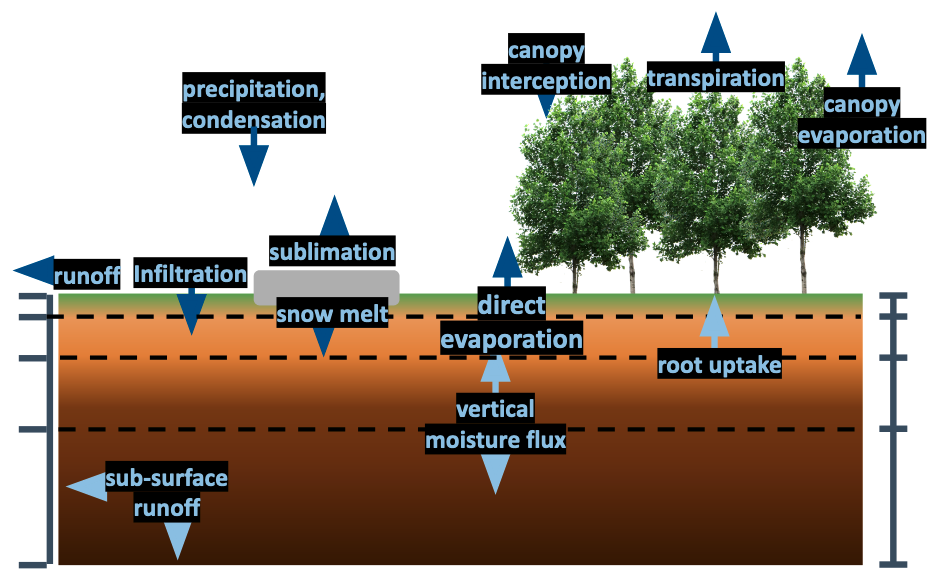
\includegraphics[width=.66\linewidth]{figures/schematic_noah-overview.png}

    \caption{Schematic diagram of the feedbacks contributing to the evolution of soil moisture in Noah-LSM}
    \label{noah-schematic}
\end{figure}

The theoretical framework underpinning Noah-LSM was initially formulated in the 1980s as part of the OSU model, which characterizes boundary layer moisture and energy fluxes as a 2-layer soil model subject to atmospheric forcings. The model expresses the infiltration and movement of water between the soil layers with the diffusive form of the Richards equation \citep{mahrt_two-layer_1984}, direct evaporation using an analytic approximation of the Penman-Montieth relation in terms of atmospheric stability \citep{mahrt_influence_1984}, and basic plant transpiration in terms of vegetation density and soil water content \citep{pan_interaction_1987}. These features form an interdependent system of differential equations that are numerically integrated using a combination of the Crank-Nicholson method and finite-differencing \citep{chen_impact_1997}, which introduces the need for short time steps of 15 or 30 minutes in order for the system to remain numerically stable \citep{cartwright_dynamics_1992}\citep{mahrt_two-layer_1984}.

The OSU model was later significantly improved, renamed to the first generation of Noah-LSM, and coupled with the NCEP Eta forecast model. Noah-LSM expanded the domain to four soil layers of increasing thicknesses (10cm, 30cm, 60cm, and 100cm), improved runoff dynamics by implementing Philip's equation for infiltration capacity \citep{schaake_simple_1996}, and represented the influence of soil texture on moisture transport by introducing bounds on bare-soil potential evaporation that are determined by the soil composition \citep{betts_assessment_1997} \citep{mahfouf_comparative_1991}. The model also features a significantly enhanced representation of vegetation including a more thorough treatment of canopy resistance via a ``Jarvis-type'' model of leaf stomatal control \citep{jarvis_interpretation_1976} \citep{jacquemin_sensitivity_1990}, which accounts for the dependence of transpiration on insolation, air temperature and dewpoint, soil moisture content, and vegetation density. The vegetation effects are scaled by a monthly climatology of normalized difference vegetation index (NDVI) values observed by the NOAA-AVHRR satellite radiometer, which serve as a proxy for green vegetation fraction (GVF) \citep{gutman_derivation_1998} \citep{chen_modeling_1996}, and the depth of root water uptake associated with plant transpiration is determined by a pixel's vegetation class as specified by the Simple Biosphere Model \citep{dorman_global_1989}. Finally, the model's utility was greatly expanded with the addition of a frozen soil and snow pack parameterization incorporating the thermal and hydraulic properties of fractionally-frozen soil layers, the effects of state changes \citep{koren_parameterization_1999}, radiative feedbacks from partial snowpack coverage, and a snow density scheme \citep{ek_implementation_2003}.

Soon after the turn of the millennium, the first generation of NLDAS was under development as part of a multi-institution collaborative effort sponsored by the Global Energy and Water Cycle Experiment (GEWEX) Continental-scale International Projects (GCIP) team. The goal of the project was to incorporate long-term observations of land surface temperature, snow pack depth, and meteorological forcings from multiple sources (in-situ, satellite, radar) into a common framework used to independently evaluate land surface states and energy fluxes with four land surface models including Noah-LSM \citep{mitchell_multi-institution_2004}. Over a domain including the full conterminous United States (CONUS) at $0.125^\circ$ resolution, the models were allowed to spin up over the course of a year, and soil states were recurrently used to initialize subsequent time steps rather than being ``nudged'' to correct for drift. Land cover and soil texture classification over the domain was derived by coarsening the University of Maryland and STATSGO datasets, respectively, from their native 1km resolutions \citep{hansen_global_2000}, surface geometry and elevation is provided by the GTOPO30 dataset \citep{earth_resources_observation_and_science_centeru_s_geological_surveyu_s_department_of_the_interior_usgs_1997}, and the parameter values for soil hydraulic properties were adapted from observations taken at the University of Virginia \citep{cosby_statistical_1984}.

\begin{table}
    \centering
    \begin{tabular}{ l l l l l}
        Forcing & Unit & Source & $\Delta$t & $\Delta$x \\
        \hline
        \multirow{2}{*}{Precipitation} & \multirow{2}{*}{kg m$^{-2}$} & CPC Gauge observations & 24h & 14km \\[-12pt]
        & & WSR-88D retrievals & 1h & 4km \\
        Temperature & K & NCEP NARR & 3h & 32km \\
        Specific Humidity & kg kg$^{-1}$ & NCEP NARR & 3h & 32km \\
        Surface Pressure & Pa & NCEP NARR & 3h & 32km \\
        Wind Velocity & m s$^{-1}$ & NCEP NARR & 3h & 32km \\
        Incident LW Flux & W m$^{-2}$ & NCEP NARR & 3h & 32km \\
        Incident SW Flux & W m$^{-2}$ & GOES, NARR & 3h, 1h & 14km \\
        Green Veg Fraction& \% & AVHRR NDVI & Monthly & 16km \\
        Leaf Area Index & m$^2$ m$^{-2}$ & UMD, AVHRR NDVI& Monthly & 16km \\
        Snow Water Equivalent & kg m$^{-2}$ & Noah-LSM & 14km \\
    \end{tabular}
    \caption{Atmospheric forcings and other time-varying parameters provided by NLDAS-2 at a 1-hourly resolution on the $0.125^\circ$ CONUS grid. Data are resampled using spatial bilinear interpolation, then temporal disaggregation according to \citep{cosgrove_real-time_2003}. NLDAS forcing files also include values for convective available potential energy, the ratio of precipitation from convection, and surface potential evaporation (calculated as in \citep{mahrt_influence_1984}), but these three values aren't currently used as inputs to the models. Snow water equivalent estimates are an output of Noah-LSM by default, but are included as a predictor here under the assumption that they can be provided from a separate model or data assimilation source.}
    \label{forcing}
\end{table}

Attention remained on Noah-LSM in the following years as it continued to support NLDAS and other data assimilation and forecasting systems, which led to a series of improvements introduced alongside the next phase of the NLDAS project. A seasonal effect was added to vegetation by scaling the leaf area index (LAI) by the GVF within bounds determined by the plant type, and transpiration was scaled by a root uptake efficiency factor determined by the proximity of soil temperature to an optimum growth temperature (298 K). Several parameters were adjusted including the influence of vapor pressure deficit on transpiration rate, the minimum stomatal resistance for several plant species, and hydraulic parameters for some soil textures. The aerodynamic conductance coefficient -- an important factor in the strength of moisture and energy fluxes from the surface -- was increased during daylight hours, and a basic anisotropy model was introduced by modifying the albedo of some surfaces in terms of the solar zenith angle \citep{wei_improvement_2011}. Snowpack physics were also modified to improve surface exchange coefficients, and to gradually diminish the snow albedo over the time since the last snowfall \citep{livneh_noah_2009} \citep{liang_simple_1994}. These changes introduce new feedbacks and involve sensitive parameters like LAI which have a strong influence on the model's dynamics \citep{rosero_quantifying_2010}. The retrospective NLDAS-2 data record generated after applying these modifications extends back to 1979, and continues to be updated in a near real-time capacity \citep{xia_continental-scale_2012}.

The NLDAS-2 time-varying retrospective forcings listed in Table \ref{forcing} will serve as the predictors used by the neural networks to forecast the Noah land surface model soil moisture states. Temperature, humidity, pressure, wind speed and heading, and longwave flux are derived exclusively from the National Centers for Environmental Prediction (NCEP) North American Regional Reanalysis (NARR) data product. As part of the downscaling procedure from their native 32km resolution to the 1/8$^\circ$ NLDAS domain, a lapse rate adjustement is applied to the temperature and humidity fields based on the elevation profile. Downward shortwave radiative flux is calculated using a blend of NARR and hourly Geostationary Operational Environmental Satellite (GOES) data, with a ratio-based bias correction based on \citep{berg_impact_2003} applied to account for a known positive bias in NARR-reported downward shortwave flux, and to mitigate discontinuities arising from the merger the two data sources \citep{pinker_surface_2003} \citep{xia_continental-scale_2012-1}. Precipitation receives a special treatment in order to ensure sufficient spatial resolution and consistency; the Climate Prediction Center (CPC) daily gauge-based product \citep{chen_assessing_2008} serves as the baseline, which is temporally disaggregated to 1 hour resolution using National Weather Service WSR-88D radar retrievals \citep{fulton_wsr-88d_1998}. In regions lacking radar coverage, the disaggregation is completed using a weighted combination of the CPC's satellite-derived estimates from morphed passive-microwave and infrared observations (CMORPH) \citep{joyce_cmorph_2004}, and the CPC Hourly Precipitation Dataset (HPD), with NARR data as a final fallback \citep{baldwin_ncep_1997}.  Although both the LAI and GVF vegetation parameters are based on multi-year monthly averages, they are disaggregated to an hourly resolution in order to be smoothly variable \citep{wei_improvement_2011}, and are thus treated like an atmospheric forcing in this work.

\section{Calibration and Validation of Noah-LSM}

During the development of Noah-LSM, researchers integrated information from a variety of observational datasets in order to calibrate and validate the soil moisture, energy flux, and radiative components of the model outputs. The initial field campaign data that bootstrapped development of the OSU model precursor came from the First International Satellite Land Surface Climatology Project Field Experiment (ISLSCP FIFE) \citep{sellers_overview_1992}, which utilized averaged evaporation data data from 10 stations in a 15x15km grassland area during the warm season of 1987. The OSU model showed strong performance in capturing the seasonal and diurnal cycle of evaporation, soil moisture, heat fluxes, and skin temperature, however struggled during wet periods due to an over-estimation of evaporation caused by the canopy resistance formulation \citep{chen_modeling_1996}.

Based on these results, others utilized further observations to integrate and parameterize new processes within Noah-LSM in order to mitigate the shortcomings. For example, and the bare surface evaporation and vegetation schemes were improved by \citep{betts_assessment_1997} based on four 48-hour intensive observation periods within FIFE, surface runoff parameters were improved by \citep{schaake_simple_1996} based on long-term USGS stream discharge datasets from gauged basins in Oklahoma, Mississippi, and North Carolina. The radiation balance and heat flux magnitudes from Noah-LSM were evaluated with respect to a full year of data from 7 sites in the Oklahoma Mesonet by \citep{sridhar_validation_2002}, who found a slight positive bias in flux magnitudes, but overall good performance with root mean squared error rates for all fluxes falling below 2.5 $MJ\,m^{-2}\,d^{-1}$. Fluxes, temperatures, radiation, and soil moisture were further validated by \citep{robock_evaluation_2003} with respect to Oklahoma Mesonet and ARM/CART surface station observations from 1998 and 1999; they found that Noah-LSM performed better than all other models in the NLDAS framework, but had a positive bias in soil moisture around 7\%, which was postulated to be the consequence of inadequacy in the static soil parameterization.

Snow and frozen soil posed a particular issue during the early development of Noah-LSM, as neglecting the physics of partially-frozen soil, fractional snow cover, and variable snow density resulted in significant underestimates in soil moisture, and high error rates in soil temperature. These shortcomings were addressed by the new physics introduced by \citep{koren_parameterization_1999}, which were calibrated based on soil moisture, temperature, and snow water equivalent observations from Rosemont, Minnesota during the 1995-1996 cold season. The ~20\% under-estimation of lower-layer soil moisture and high error in soil temperature were greatly diminished as a consequence of the changes. Significant snowpack volume under-estimates were also addressed by \citep{livneh_noah_2009} using SNOTEL station snow water equivalent data, and subsequently by \citep{barlage_noah_2010} based on problems noted by \citep{pan_snow_2003} using both SNOTEL and SNODAS data. In combination, these process improvements reduced the low bias to about 15\%, and improved the snow water equivalent correlation with the observations to about 80\%.

In the lead-up to the second generation of NLDAS, \citep{wei_improvement_2011} implemented further improvements to warm-season processes which were validated based on ARM/CART surface flux stations as well as GOES satellite retrivals of land surface temperature during the 1998 and 1999 warm seasons. The consequence was a reduction in spring-season positive bias in latent from 80 $W\,m^{-2}$ to about 20 $W\,m^{-2}$ and land surface temperature with a correlation of about .85, a slight negative bias of $-1.26\,K$, and root mean squared error around $3.08\,K$. Additionally, \citep{xia_evaluation_2014} validated NLDAS-2 modeled soil moisture against 20 years of monthly data from the Illinois climate network (1986-2004), 6 years of daily data over 72 sites from the Oklahoma Mesonet (1997-2002), and 8 years of daily data from 121 SCAN sites (2002-2009). They found that Noah exhibited a mean monthly anomaly correlation of .82 in the first 2m, which was stronger in the warms seeason but struggled when the ground was frozen or snow was present, especially in lower two soil layers. The daily mean anomaly correlation from the Oklahoma Mesonet data was greater than .8 in the lower layers and .77 in the surface layer, while the monthly averages were all above .85 with about 15\% relative MAE and a relative bias around -15% for all three tested layers. Regional analyses with respect to the widely-dispersed SCAN stations indicate substantial variability in performance; Noah-LSM struggled with the surface layers in the Northeast US with a correlation of only about .2, but was consistently better than .5 correlation elsewhere, especially in the Great Plains and Northwest. The midwest also exhibited a large dry bias, which is likely the consequence of a lack of irrigation information in the cropland-dominated region.

Finally, an entropy-based decomposition of uncertainty was employed by \citep{nearing_benchmarking_2016} to quantify the components of error in Noah-LSM caused by improper characterization of forcings, model dynamical structures, and model parameters. By comparing to soil moisture observations from 49 SCAN sites and 50 AmeriFlux stations active between 2001 and 2011, they determined that inadequate model parameters like soil texture and vegetation classification were the greatest sources of uncertainty in the soil moisture profile, while biased input forcings were the dominant cause of uncertainty for energy fluxes.

\section{Distinctions in Modeling Techniques}

\begin{figure}[h]
    \centering

    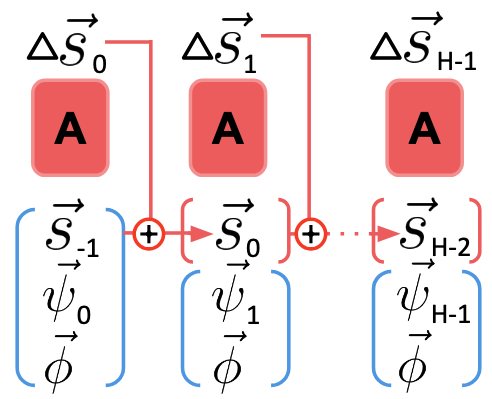
\includegraphics[width=.66\linewidth]{figures/schematic_scann.png}

    \caption{Diagram of a self-cycling discrete-time dynamical system with no hidden state. At each time, nonlinear operator \textbf{A} maps an initial state $\vec{s}_{k-1}$, exogenous forcing $\vec{\psi}_k$, and time-invariant parameters $\vec{\phi}$ to a new state $\Delta \vec{s}_k$, used to initialize the subsequent time step, and so forth until $H$ predictions have been made.}
    \label{scann}
\end{figure}

\subsection{Noah-LSM as a Discrete Dynamical System}

At its core, Noah-LSM is a collection of coupled differential equations that express the total derivative of land surface states $\frac{d\vec{s}}{dt}$ in terms of the current state $\vec{s}$, forcing $\vec{\psi}$, and time-invariant properties of each grid cell $\vec{\phi}$. Since the model is implemented as an algorithmic procedure and is not continuously differentiable, we will use the notation $\frac{\Delta \vec{s}_k}{\Delta t} \approx \mathbf{A}(\vec{s}_{k-1}, \vec{\psi}_k, \vec{\phi}, \Delta t)$ to refer to the model as a transition function evaluated at a discrete time step $\Delta t$, such that the system evolves as a dynamical system described by Equation \ref{dynamical}.

\begin{equation}\label{dynamical}
    \vec{s}_k = \vec{s}_{k-1} + \mathbf{A}(\vec{s}_{k-1}, \vec{\psi}_k, \vec{\phi}_k, \Delta t) \cdot \Delta t
\end{equation}

Here, $\vec{s}_k$ refers to the model's dynamic state variables like snow pack depth, soil moisture and temperature, and canopy storage, $\vec{\psi}_k$ encodes the covariate atmospheric variables from Table \ref{forcing} (which are derived from weather forecasts or observations), and $\vec{\phi}$ includes time-invariant coefficients of the governing equations like vegetation type/fraction, soil texture, and slope/elevation. As a matter of convention, the time step $k=0$ refers to the first perturbation of the initial state after applying the model's first increment change estimate, and includes the forcings that informed that perturbation, consistent with the relationships depicted by Figure \ref{scann}.

To generate a time series, Noah-LSM numerically integrates the system of equations using Euler and Crank-Nicholson techniques, which explicitly evaluate the differential equations at several time intervals per computational time step in order to estimate the nonlinear change in state, which evolves continuously in the real system being modeled. It is crucial that the increment change in time remains small between evaluations of the model (15min for NLDAS-Noah) to mitigate truncation error from the assumption of local linearity \citep{mitchell_multi-institution_2004} \citep{cartwright_dynamics_1992}. As Figure \ref{scann} suggests, the model does not retain any ``hidden'' internal information that is updated between timesteps; at each point, the information available to determine the new change in state is limited to the input domain of the model.

\subsection{Process-based vs Data-driven Models}

The process-based approach of numerical models like Noah-LSM is practically and epistemologically distinct from data-driven techniques like deep learning. In a process-based paradigm, the inductive biases that govern the model's behaviors can be explicitly understood since they are based on a characterization of the physical system which is derived from theoretical knowledge. Some uncertainty is introduced by the input data, and is shared among all model types; this includes uncertainty from noise and interpolation of forcing observations, discrete treatment of surface types, etc. Aside from that, model error in process-based models arises from sources including inadequacy of the theory for describing the system (that is, phenomena which are neglected or misrepresented, and become a source of unexplained variance), and truncation error accumulated from the approximation techniques used to solve the model's governing equations. Explicit understanding of the reasons for the model's behavior has the advantage of being interpretable, in the sense that particular systems within the model can be independently evaluated and blamed for contributing uncertainty. Additionally, granting the ability to impose absolute constraints within the model structure ensures the outputs fully adhere to some physical requirements, such as conservation of water and energy. Nonetheless, the onus falls entirely on the model developer to adjust many details of the implementation of the processes. The act of tuning a numerical model's parameters often implies postulating a source of uncertainty, addressing it by manually manipulating coefficients or introducing new systems within the governing equations, and then evaluating the impact of the changes using correlational analysis with a subset of the available data. This can be a laborious process, and typically results in the gradual accumulation of feedbacks and complexity within the model.

In contrast, many data-driven approaches to modeling physical systems -- deep learning in particular -- sacrifice the explainability and rigorous physicality of their estimates in exchange for developing a statistically optimal approximation of the relationship between the input and output domains by any means available. Although the overall algorithmic structure of the ANN is established by the developer -- typically based on broad heuristics from past literature and experimentation -- very little control can be asserted over the particular means by which predictions are determined from inputs. Instead, the effectiveness of the ANN's performance is characterized in terms of a differentiable loss function (also known as the objective or cost function) which may be defined by the developer, and which is fundamentally (though indirectly) important for determining the solution developed in the training phase.

An ANN's learnable parameters refer to the real-valued elements of a series of arbitrarily-sized square matrices encoding affine transformations. Each ``layer'' of the ANN is comprised of one of these affine transformations followed by an element-wise nonlinear operation on its output, and the full ANN typically consists of multiple layers which are combined via composition or any kind of differentiable arithmetic operation. During training, all of the ANN's learnable parameters are iteratively adjusted by estimating the gradient of the loss function with respect to the parameters (given batched subsets of the predictor/target data pairs) then determining the direction and magnitude by which the parameters in each of the layers should be modified with an algorithm called backpropagation \citep{rumelhart_learning_1986}. The general strategy of determining the sensitivity of the loss landscape to changes in the ANN's parameters, and tweaking them accordingly, is referred to as gradient descent. Given at least 2 layers (which constitutes the definition of a \textit{deep} ANN), the network is theoretically capable of expressing an arbitrary decision boundary or multivariate function given a sufficient number of parameters \citep{hornik_multilayer_1989}. This high level of expressivity enables the network to learn complex relationships and generalizations among high-dimensional parameters, given repeated exposure to instances of these relationships during training.

The principle of ANNs using high-dimensional nonlinear correlations rather than explicit processes to model the correspondence between two datasets is powerful because they can approximate a highly nonlinear regression without numerically integrating a complex algorithm, and they can learn their parameterization based on a large volume of data without manual intervention. The quintessential drawback of relying on a black-box approach, though, is that models may perform poorly for no apparent reason, or may perform well for a fraught reason. For example, in one commonly-invoked anecdote described by \citep{lapuschkin_unmasking_2019}, an image classifier over-performing but failing to generalize at identifying horses in a grassy field was found to actually rely on the presence of the watermark of a particular equestrian photographer whose work was a part of the training data. As such, only regarding bulk statistics and loss performance as indicative of a model's success is insufficient to consider it trustworthy. In a data-driven paradigm, then, the role of the ANN developer is to facilitate effective and reliable learning through careful training data curation, congnizant loss function and model architecture design, and thorough evaluation of the model's behavior in local and global scenarios throughout the input domain in order to ensure the effectiveness and consistency of predictions in a variety of inference settings.

Furthermore, it is important to note that in the current scope of this work, it is not possible for the ANNs to leverage their expressivity to out-perform the numerical model. Since the ANNs presented here are merely emulating the processes that are programmed into Noah-LSM, it isn't reasonable to expect the models to form a more accurate representation of real soil dynamics. Nonetheless, it is conceivable that future work could utilize a similar approach to \citep{o_global_2021} in order to integrate observational data into the training domain alongside model data, or to use it as a prediction target. The merger of these two data sources could aid in improving a data-driven model beyond the limitations of a numerical model's structure.

\section{Deep Learning of Time Series}

\begin{figure}[h!]
    \centering

    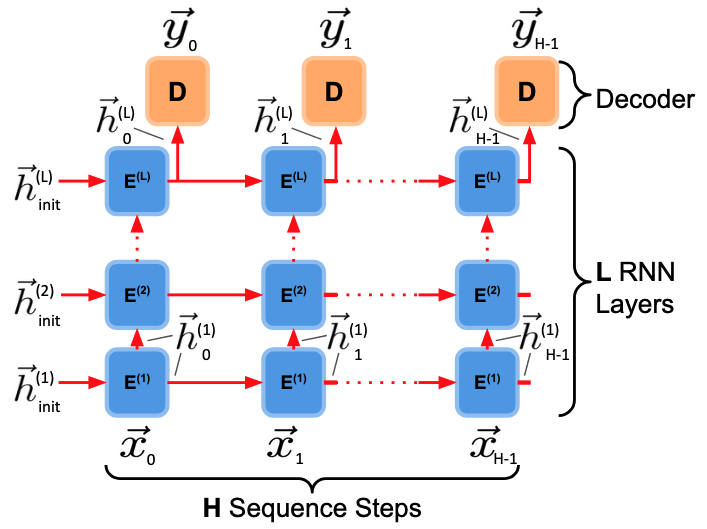
\includegraphics[width=.95\linewidth]{figures/schematic_abstract-rnn.png}

    \caption{Schematic representation of an abstract sequence-to-sequence RNN with multiple layers.}
    \label{schematic-rnn}
\end{figure}

The most simple variant of an ANN is referred to as a feed-forward neural network (FNN), which consists of a series of composed layers (see previous section) mapping the input vector directly to the output. Although a FNN is theoretically capable of simulating Noah-LSM in the manner of Figure \ref{scann}, inductive biases are commonly introduced in model architectures in order to promote efficiency, explainability, stability, and parsimony. For example, most neural networks used for sequence modeling like the recurrent neural networks (RNNs) in Figure \ref{schematic-rnn} maintain one or more ``hidden'' latent parameters $\vec{h}$ with an arbitrary number of dimensions. This vector is modified and passed along by each subsequent iteration, giving the network the ability to make temporal generalizations and propagate information to future predictions. Although $\vec{h}$ is typically difficult to interpret directly, the gradient descent process incentivizes the network to preserve and consolidate information that is needed to accurately generate the full sequence of predictions. This construct is promising for improving the models' ability to estimate soil dynamics because characteristic drydown curves are known to exhibit hysteresis depending on their recent patterns of wetting and drying \citep{haines_studies_1930}. %Each of the following network architectures ultimately aim to improve the information quality of the latent vector by implementing algebraic structure, introducing statistical uncertainty, and encouraging sparsity.

\begin{equation}\label{eq_rnn}
    \begin{split}
        %\vec{h}_k^{(1)} &= \mathbf{E^{(1)}}\left(\vec{h}_{k-1}^{(1)},\, \vec{\psi}_k,\, \vec{\phi}\right) \\
        \vec{h}_k^{(1)} &= \mathbf{E^{(1)}}\left(\vec{h}_{k-1}^{(1)},\, \vec{x}_k\right) \\
        \vec{h}_k^{(j)} &= \mathbf{E^{(j)}}\left(\vec{h}_{k-1}^{(j)},\, \vec{h}_k^{(j-1)}\right) \\
        \vec{y}_k &= \mathbf{D}\left(h_k^{(L)}\right)
        %\vec{s}_{k+1} &= \vec{s}_{k} + \mathbf{D}\left(h_k^{(L)}\right)
    \end{split}
\end{equation}

The RNNs discussed here will follow the general structure described by Equation \ref{eq_rnn}, which is consistent with the abstract architecture diagrammed in Figure \ref{schematic-rnn}, and follows the typical approach for constructing RNNs as outlined in \citep{russell_artificial_2020}. The architecture consists of L encoder layers (\textbf{E}$^{(1)}$-\textbf{E}$^{(L)}$) which generate H top-layer latent vectors corresponding to each of the prediction times, and 1 layer of decoder weights \textbf{D} which converts each of the top-layer latent vectors to a prediction for the increment change in state $\Delta \vec{s}$ between the current timestep and the next one. Parameters for \textbf{E} and \textbf{D} are shared across timesteps, however each of the L layers have distinct parameters. Here, $\vec{h}_k^{(1)}$ is a member of the time series of first-layer latent vectors given the arguments $\vec{x}_k$ and the latent vector from the previous first-layer timestep $\vec{h}_{k-1}^{(1)}$. Moving upward, $\vec{h}_k^{(j)}$ is an intermediate-layer latent vector such that $j \in [2,\,L]$, and when $k=0$ (the first horizon timestep), $\vec{h}^{(s)}_{-1} = \vec{h}^{(s)}_{\text{init}}$ for any layer $s$. In many cases, the initial hidden states $\vec{h}^{(s)}_{init}$ are randomized or set to zero, however in this project we use a separate spin-up RNN to establish them, as will be discussed in the Methodology section.

\begin{figure}[h!]
    \centering

    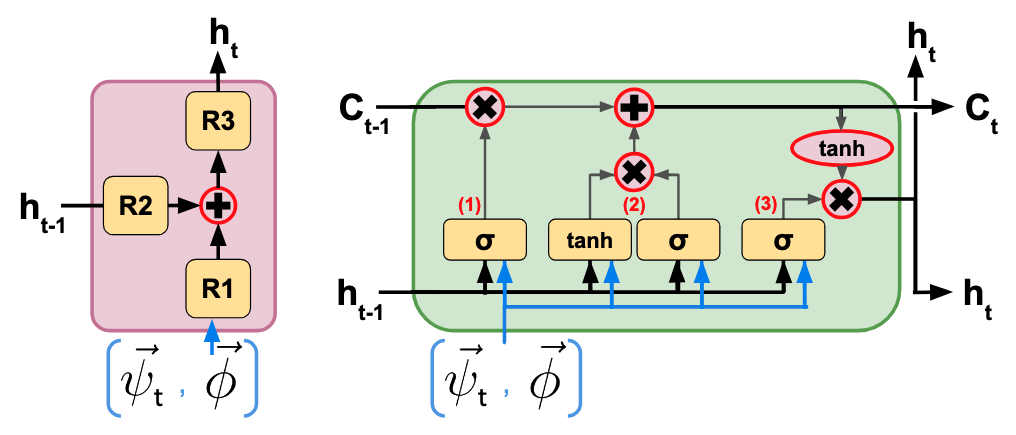
\includegraphics[width=.95\linewidth]{figures/schematic_rnns-both.png}

    \caption{Schematic representation of individual RNN cells, the na\"ive RNN (left), and the LSTM (right)}
    \label{rnns-both}
\end{figure}

The term RNN does not refer to a specific neural network architecture, but rather the category of architectures that share their weights across sequence steps. The sub-network unit of weights applied at each timestep (\textbf{G} or \textbf{E} in Figure \ref{s2s-default}) is referred to as a RNN cell, and must contain internal structure for converting inputs from lower layers and the previous timestep into an output. Unlike traditional ANNs which use backpropagation to train on single input-output pairs, each cell must balance the penalty of its loss gradient between contributions from the input at each timestep with contributions from the latent vector of the previous timestep. To accommodate this difference, RNNs are trained using a special type of gradient descent called backpropagation through time, which balances the loss with respect to the two input sources, and accumulates it across all timesteps before updating each cell's parameters.

The most basic form of the RNN architecture (diagrammed on the left side of Figure \ref{rnns-both}) consists of 3 separate affine operations. As shown in the figure, R1 and R2 convert the lower-layer and previous-timestep vectors, respectively, into two uniformly-sized internal latent vectors. The sum of these internal vectors are transformed by a third affine operation, R3, into the cell's output, which is passed along to the higher layer and subsequent steps within the same layer.

This style of na\"ive RNN is vulnerable to the so-called vanishing or exploding gradient problem, which arises from the fact that the cell output is the direct product of learned matrix operations. Since during training each cell's weights are updated recurrently based on many sequence steps, the loss gradient with respect to each learned parameter can become incredibly sensitive to changes in each parameter. This can cause weights to become very close to zero, or to diverge to very large numbers, which halts the learning process \citep{mozer_focused_1995}. Furthermore, since the latent state passed between sequence steps undergoes a nonlinear transformation at each instance of the cell, it is more tenuous for the network to sustain information over a long context of past observations.

The LSTM architecture addresses these shortcomings by maintaining a separate hidden state $\vec{C}_t$ called the context vector. Rather than being generated by a matrix operation at each step, the context vector is only modified from the previous step's value using the output of a series of three ``gates.'' These gates (numbered in Figure \ref{rnns-both})  include (1) the ``forget gate'', which uses a FNN to select a vector of values in the range (0,1). The forget vector is multiplied element-wise by $\vec{C}_{t-1}$ in order to selectively emphasize or diminish its activation. The ``update gate'' (2) transforms the inputs into a new coefficient vector in the range (-1,1), which is added to the context vector in order to retain information from the current time step. Finally, the ``output gate'' (3) generates a vector of multiplicative coefficients in the range (0,1) used to scale the new context vector $\vec{C}_t$ to the output latent state $\vec{h}_t$ \citep{hochreiter_long_1997}. The context vector remains stable compared to a hidden vector that is recurrently operated on by the same weight matrix, which facilitates the network to learn over a longer sequence interval.

The Transformer architecture has dominated many sequence modeling tasks in recent literature thanks to the key innovation of multi-head self-attention (MSA), which enables the architecture to learn complicated relationships between individual members of the input sequence regardless of their relative position. Additionally, transformers are efficient to train in parallel, unlike RNN architectures which rely on a chain of sequential operations, which makes them straightforward to train on a massive scale \citep{vaswani_attention_2017}. The results for natural language processing (NLP) \citep{devlin_bert_2019} and image classification \citep{dosovitskiy_image_2021} tasks are impressive, however there are several key drawbacks that make them less appealing for a time series generation task like this one.

First, the memory cost of a transformer scales quadratically with sequence length since MSA learns parameters relating every possible combination of input steps. This is compounded with the fact that the full input sequence needs to be re-initialized with every step during inference. These properties are a direct trade-off with the Transformer's ability to train separate sequence steps in parallel. Furthermore, unlike RNNs and CNNs, Transformers don't have an inherent notion of order. In problems like NLP where sequence position conveys some information, a simple form of locality is introduced by adding a positional embedding vector directly to the inputs. Prior literature shows that transformers equipped with positional embedding still perform no better on basic time series forecasting tasks than a simple 2-layer FNN \citep{zeng_are_2022}. For these reasons, although MSA is a very powerful tool for many applications, we will be neglecting this very popular architecture in this work.

\chapter{Chapter 3. Data and Methodology}

\begin{table}[ht]

\caption[Frequencies for equal-tempered scale, $A_4=440$]{Frequencies for equal-tempered scale, $A_4=440$ Hz. This table shows only the first five notes of a chromatic scale starting on $C_0$} %Just provide the title of the table in the square brackets. Then, in the next set of brackets, provide the entire caption (including the title again). By doing this, only the title of the table will be on the List of Tables instead of the entire caption. The first sentence of the caption can be the title.

\begin{center}
\resizebox{\columnwidth}{!}{
\begin{tabular}{|c | c | c |}
 \hline
\textbf{Note} & \textbf{Frequency (Hz)} & \textbf{Wavelength} \\ [0.5ex]
 \hline
 $C_0$ & 16.35 & 2109.89 \\
 \hline
 $C^{\#}_0/D^b_0$ & 17.32 & 1991.47 \\
 \hline
 $D_0$ & 18.35 & 1879.69 \\
 \hline
 $D^{\#}_0/E^b_0$ & 19.45 & 1774.20 \\
 \hline
 $E_0$ & 20.60 & 1674.62 \\ [1ex]
 \hline
\end{tabular}
}
\end{center}


\end{table}



%************************
%Back Matter of your Thesis Begins
%************************
\backmatter

%***********************
%References
%***********************
\addcontentsline{toc}{chapter}{References} %This adds the Bibliography/References to your table of contents.
\bibliographystyle{apalike} %This selects your bibliography style. There are many possible bibliography styles you can choose. The following site explains the options. https://www.overleaf.com/learn/latex/Bibtex_bibliography_styles


\begingroup %Begins an editable environment to set proper spacing for the bibliography/references page.
\setlength{\bibsep}{12pt} %This provides 10 pts between reference entries.
\setstretch{1} %This specifies single-spacing within entries.
\bibliography{dodson_masters-thesis} %This inserts your References. You must individually add all references to the ref.bib file. Then, only those references you actually cite in the body of your text will be included.
\endgroup

%***********************
%Appendix Section: Optional. If you do not want to include any appendices, simply delete the below commands that create the appendix environment and that input your appendix file(s).
%**********************
\appendix %This creates the appendix environment.

\chapter{Appendix A: An Example Appendix}%Be sure to include the Heading Appendix A: before you type the name of the Appendix.

\renewcommand{\thechapter}{A} %If you add another appendix, copy and paste this line, but update it to B instead of A.

Appendices should appear at the very end of your thesis. Make sure to label each Appendix with a letter starting with "A". Any tables and/or figures located in the appendix should be labeled accordingly. For example, below is figure A.1 because it is the first figure that appears in Appendix A. 


\begin{figure}[ht]
    \centering
    \includegraphics[width=\textwidth]{Figures/Figure A.1.png}
    \caption[Colleges and Universities in Alabama]{Colleges and Universities in Alabama}
    \label{fig a.1}
\end{figure}


 %This inserts your Appendix file(s). To edit this page, open the Appendix A.tex file. You will need to create a new .tex file for each appendix you want to include.

\end{document}
